% Options for packages loaded elsewhere
\PassOptionsToPackage{unicode}{hyperref}
\PassOptionsToPackage{hyphens}{url}
\PassOptionsToPackage{dvipsnames,svgnames,x11names}{xcolor}
%
\documentclass[
  letterpaper,
  DIV=11,
  numbers=noendperiod]{scrartcl}

\usepackage{amsmath,amssymb}
\usepackage{iftex}
\ifPDFTeX
  \usepackage[T1]{fontenc}
  \usepackage[utf8]{inputenc}
  \usepackage{textcomp} % provide euro and other symbols
\else % if luatex or xetex
  \usepackage{unicode-math}
  \defaultfontfeatures{Scale=MatchLowercase}
  \defaultfontfeatures[\rmfamily]{Ligatures=TeX,Scale=1}
\fi
\usepackage{lmodern}
\ifPDFTeX\else  
    % xetex/luatex font selection
\fi
% Use upquote if available, for straight quotes in verbatim environments
\IfFileExists{upquote.sty}{\usepackage{upquote}}{}
\IfFileExists{microtype.sty}{% use microtype if available
  \usepackage[]{microtype}
  \UseMicrotypeSet[protrusion]{basicmath} % disable protrusion for tt fonts
}{}
\makeatletter
\@ifundefined{KOMAClassName}{% if non-KOMA class
  \IfFileExists{parskip.sty}{%
    \usepackage{parskip}
  }{% else
    \setlength{\parindent}{0pt}
    \setlength{\parskip}{6pt plus 2pt minus 1pt}}
}{% if KOMA class
  \KOMAoptions{parskip=half}}
\makeatother
\usepackage{xcolor}
\setlength{\emergencystretch}{3em} % prevent overfull lines
\setcounter{secnumdepth}{-\maxdimen} % remove section numbering
% Make \paragraph and \subparagraph free-standing
\ifx\paragraph\undefined\else
  \let\oldparagraph\paragraph
  \renewcommand{\paragraph}[1]{\oldparagraph{#1}\mbox{}}
\fi
\ifx\subparagraph\undefined\else
  \let\oldsubparagraph\subparagraph
  \renewcommand{\subparagraph}[1]{\oldsubparagraph{#1}\mbox{}}
\fi

\usepackage{color}
\usepackage{fancyvrb}
\newcommand{\VerbBar}{|}
\newcommand{\VERB}{\Verb[commandchars=\\\{\}]}
\DefineVerbatimEnvironment{Highlighting}{Verbatim}{commandchars=\\\{\}}
% Add ',fontsize=\small' for more characters per line
\usepackage{framed}
\definecolor{shadecolor}{RGB}{241,243,245}
\newenvironment{Shaded}{\begin{snugshade}}{\end{snugshade}}
\newcommand{\AlertTok}[1]{\textcolor[rgb]{0.68,0.00,0.00}{#1}}
\newcommand{\AnnotationTok}[1]{\textcolor[rgb]{0.37,0.37,0.37}{#1}}
\newcommand{\AttributeTok}[1]{\textcolor[rgb]{0.40,0.45,0.13}{#1}}
\newcommand{\BaseNTok}[1]{\textcolor[rgb]{0.68,0.00,0.00}{#1}}
\newcommand{\BuiltInTok}[1]{\textcolor[rgb]{0.00,0.23,0.31}{#1}}
\newcommand{\CharTok}[1]{\textcolor[rgb]{0.13,0.47,0.30}{#1}}
\newcommand{\CommentTok}[1]{\textcolor[rgb]{0.37,0.37,0.37}{#1}}
\newcommand{\CommentVarTok}[1]{\textcolor[rgb]{0.37,0.37,0.37}{\textit{#1}}}
\newcommand{\ConstantTok}[1]{\textcolor[rgb]{0.56,0.35,0.01}{#1}}
\newcommand{\ControlFlowTok}[1]{\textcolor[rgb]{0.00,0.23,0.31}{#1}}
\newcommand{\DataTypeTok}[1]{\textcolor[rgb]{0.68,0.00,0.00}{#1}}
\newcommand{\DecValTok}[1]{\textcolor[rgb]{0.68,0.00,0.00}{#1}}
\newcommand{\DocumentationTok}[1]{\textcolor[rgb]{0.37,0.37,0.37}{\textit{#1}}}
\newcommand{\ErrorTok}[1]{\textcolor[rgb]{0.68,0.00,0.00}{#1}}
\newcommand{\ExtensionTok}[1]{\textcolor[rgb]{0.00,0.23,0.31}{#1}}
\newcommand{\FloatTok}[1]{\textcolor[rgb]{0.68,0.00,0.00}{#1}}
\newcommand{\FunctionTok}[1]{\textcolor[rgb]{0.28,0.35,0.67}{#1}}
\newcommand{\ImportTok}[1]{\textcolor[rgb]{0.00,0.46,0.62}{#1}}
\newcommand{\InformationTok}[1]{\textcolor[rgb]{0.37,0.37,0.37}{#1}}
\newcommand{\KeywordTok}[1]{\textcolor[rgb]{0.00,0.23,0.31}{#1}}
\newcommand{\NormalTok}[1]{\textcolor[rgb]{0.00,0.23,0.31}{#1}}
\newcommand{\OperatorTok}[1]{\textcolor[rgb]{0.37,0.37,0.37}{#1}}
\newcommand{\OtherTok}[1]{\textcolor[rgb]{0.00,0.23,0.31}{#1}}
\newcommand{\PreprocessorTok}[1]{\textcolor[rgb]{0.68,0.00,0.00}{#1}}
\newcommand{\RegionMarkerTok}[1]{\textcolor[rgb]{0.00,0.23,0.31}{#1}}
\newcommand{\SpecialCharTok}[1]{\textcolor[rgb]{0.37,0.37,0.37}{#1}}
\newcommand{\SpecialStringTok}[1]{\textcolor[rgb]{0.13,0.47,0.30}{#1}}
\newcommand{\StringTok}[1]{\textcolor[rgb]{0.13,0.47,0.30}{#1}}
\newcommand{\VariableTok}[1]{\textcolor[rgb]{0.07,0.07,0.07}{#1}}
\newcommand{\VerbatimStringTok}[1]{\textcolor[rgb]{0.13,0.47,0.30}{#1}}
\newcommand{\WarningTok}[1]{\textcolor[rgb]{0.37,0.37,0.37}{\textit{#1}}}

\providecommand{\tightlist}{%
  \setlength{\itemsep}{0pt}\setlength{\parskip}{0pt}}\usepackage{longtable,booktabs,array}
\usepackage{calc} % for calculating minipage widths
% Correct order of tables after \paragraph or \subparagraph
\usepackage{etoolbox}
\makeatletter
\patchcmd\longtable{\par}{\if@noskipsec\mbox{}\fi\par}{}{}
\makeatother
% Allow footnotes in longtable head/foot
\IfFileExists{footnotehyper.sty}{\usepackage{footnotehyper}}{\usepackage{footnote}}
\makesavenoteenv{longtable}
\usepackage{graphicx}
\makeatletter
\def\maxwidth{\ifdim\Gin@nat@width>\linewidth\linewidth\else\Gin@nat@width\fi}
\def\maxheight{\ifdim\Gin@nat@height>\textheight\textheight\else\Gin@nat@height\fi}
\makeatother
% Scale images if necessary, so that they will not overflow the page
% margins by default, and it is still possible to overwrite the defaults
% using explicit options in \includegraphics[width, height, ...]{}
\setkeys{Gin}{width=\maxwidth,height=\maxheight,keepaspectratio}
% Set default figure placement to htbp
\makeatletter
\def\fps@figure{htbp}
\makeatother

\usepackage{physics}
\KOMAoption{captions}{tableheading}
\makeatletter
\@ifpackageloaded{caption}{}{\usepackage{caption}}
\AtBeginDocument{%
\ifdefined\contentsname
  \renewcommand*\contentsname{Table of contents}
\else
  \newcommand\contentsname{Table of contents}
\fi
\ifdefined\listfigurename
  \renewcommand*\listfigurename{List of Figures}
\else
  \newcommand\listfigurename{List of Figures}
\fi
\ifdefined\listtablename
  \renewcommand*\listtablename{List of Tables}
\else
  \newcommand\listtablename{List of Tables}
\fi
\ifdefined\figurename
  \renewcommand*\figurename{Figure}
\else
  \newcommand\figurename{Figure}
\fi
\ifdefined\tablename
  \renewcommand*\tablename{Table}
\else
  \newcommand\tablename{Table}
\fi
}
\@ifpackageloaded{float}{}{\usepackage{float}}
\floatstyle{ruled}
\@ifundefined{c@chapter}{\newfloat{codelisting}{h}{lop}}{\newfloat{codelisting}{h}{lop}[chapter]}
\floatname{codelisting}{Listing}
\newcommand*\listoflistings{\listof{codelisting}{List of Listings}}
\makeatother
\makeatletter
\makeatother
\makeatletter
\@ifpackageloaded{caption}{}{\usepackage{caption}}
\@ifpackageloaded{subcaption}{}{\usepackage{subcaption}}
\makeatother
\ifLuaTeX
  \usepackage{selnolig}  % disable illegal ligatures
\fi
\usepackage[]{biblatex}
\usepackage{bookmark}

\IfFileExists{xurl.sty}{\usepackage{xurl}}{} % add URL line breaks if available
\urlstyle{same} % disable monospaced font for URLs
\hypersetup{
  pdftitle={Eigensolver},
  pdfauthor={Elisabeth Welizky},
  colorlinks=true,
  linkcolor={blue},
  filecolor={Maroon},
  citecolor={Blue},
  urlcolor={Blue},
  pdfcreator={LaTeX via pandoc}}

\title{Eigensolver}
\author{Elisabeth Welizky}
\date{2024-10-01}

\begin{document}
\maketitle

\renewcommand*\contentsname{Table of contents}
{
\hypersetup{linkcolor=}
\setcounter{tocdepth}{3}
\tableofcontents
}
\section{Introduction}\label{introduction}

In this work we discuss an Eigensolver, which aims to find the lowest
Eigenvalue of a given Electronic Hamiltonian. To briefly recap: A
Hamiltonian itself describes the possible energies of a physical system,
including both the kinetic and potential energy of that system and is
represented by a matrix. If we know the Hamiltonian, we can gain
information about the physical states of the system. In our example, the
Hamiltonian takes the following form

\begin{Shaded}
\begin{Highlighting}[]
\ImportTok{import}\NormalTok{ tequila }\ImportTok{as}\NormalTok{ tq}
\ImportTok{import}\NormalTok{ numpy }\ImportTok{as}\NormalTok{ np}
\NormalTok{H }\OperatorTok{=} \FloatTok{1.5}\OperatorTok{{-}}\FloatTok{0.5}\OperatorTok{*}\NormalTok{(tq.paulis.Z(}\DecValTok{1}\NormalTok{)}\OperatorTok{{-}}\NormalTok{tq.paulis.Z(}\DecValTok{0}\NormalTok{)}\OperatorTok{+}\NormalTok{tq.paulis.Z(}\DecValTok{0}\NormalTok{)}\OperatorTok{*}\NormalTok{tq.paulis.Z(}\DecValTok{1}\NormalTok{)}\OperatorTok{+}\NormalTok{tq.paulis.X(}\DecValTok{1}\NormalTok{)}\OperatorTok{{-}}\NormalTok{tq.paulis.Z(}\DecValTok{0}\NormalTok{)}\OperatorTok{*}\NormalTok{tq.paulis.X(}\DecValTok{1}\NormalTok{))}
\end{Highlighting}
\end{Shaded}

Since we can regard the Hamiltonian as a Hermition Operator we can write
it as follows:\\
\[H\ket{\Psi_{guess}} =  E_{guess}\ket{\Psi_{guess}} \iff E_{guess} = \bra{\Psi_{guess}}H\ket{\Psi_{guess}}.\]
Now \(E_{guess}\) is the expectation value of the given Hamiltonian.

Our goal is to find such an energy \(E_{0}\) of the ground state, such
that no other energy is greater than \(E_{0}\). Therefore we need to
minimize \(E_{guess}\) to get as close as possible to the ground state
energy. In our case the seeked Eigenvalue is the angle of the minimum
Eigenstate, which corresponds to the seeked ground state energy and
which can be found by applying a minimization method on the expectation
value \(E_{guess}\).

In the following graphic we can see the plotted Hamiltonian depending on
the angle \(\phi\).

\includegraphics[width=4.16667in,height=\textheight]{Hamiltonian.png}

The circles in this graph are representinng the seeked Eigenstates of
\(H\). Therefore the corresponging angles are the seeked Eigenvalues. It
is essential to point out that minima and maxima of this graph are
potential Eigenvalues, but don´t neccessary need to be. Particularly,
when applying different excited state methods one depending on each
another, the true Eigenvalues will emerge. Therefore it is also possible
to get some potential Eigenvalues at first, which will later turn out as
irrelevant. On the other hand saddle points in the beginning might
develop to minima or maxima when applying the minimization on multiple,
consecutively executed excited state methods.

\section{Ansatz}\label{ansatz}

An Ansatz is the parameterized quantum circuit, which, in our case, we
are going to define as follows:

\begin{Shaded}
\begin{Highlighting}[]
\NormalTok{a }\OperatorTok{=}\NormalTok{ tq.Variable(}\StringTok{"a"}\NormalTok{)}
\NormalTok{U }\OperatorTok{=}\NormalTok{ tq.gates.Ry(angle}\OperatorTok{=}\NormalTok{(a)}\OperatorTok{*}\NormalTok{np.pi,target}\OperatorTok{=}\DecValTok{0}\NormalTok{)}
\NormalTok{U}\OperatorTok{+=}\NormalTok{ tq.gates.CNOT(}\DecValTok{0}\NormalTok{,}\DecValTok{1}\NormalTok{)}
\NormalTok{U}\OperatorTok{+=}\NormalTok{ tq.gates.Ry(angle}\OperatorTok{=}\NormalTok{(a}\OperatorTok{/}\DecValTok{2}\NormalTok{)}\OperatorTok{*}\NormalTok{np.pi, target}\OperatorTok{=}\DecValTok{1}\NormalTok{)}
\end{Highlighting}
\end{Shaded}

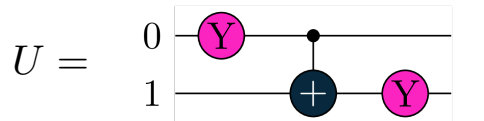
\includegraphics[width=4.16667in,height=\textheight]{circuit.png}

Since the Ansatz is an educated guess, the circuit can always be changed
until we reach an optimal solution. In this case the circuit depends on
one angle a. When modeling the minimization in a 2D-model we might also
use two different angles.

\section{Excited state methods}\label{excited-state-methods}

After having introduced the main goal and concept, we should make clear
how two implement and use those different excited state methods, given
the Hamiltonian and our computed cuircit \(U\) depending on the angles
\(\phi\). These particularly differ in the way of defining the
expectation value, with the given Hamiltonian and cuircit, as well as
the superposition of those with the correct parametrization of our given
cuircit. First we take a look at the popular ``Folded spectrum'' method.
The general form looks like this: \(<(H-\mu)^2>_{U(\phi)}\) with \(\mu\)
being a constant, in our case initially assigned to 1.\\

\begin{Shaded}
\begin{Highlighting}[]
\KeywordTok{def}\NormalTok{ expectation\_value\_folded\_spectrum(H,U, constant):}
    \ControlFlowTok{return}\NormalTok{ tq.ExpectationValue(H}\OperatorTok{=}\NormalTok{(H}\OperatorTok{{-}}\NormalTok{constant)}\OperatorTok{**}\DecValTok{2}\NormalTok{, U}\OperatorTok{=}\NormalTok{U)}
\end{Highlighting}
\end{Shaded}

The next method is the appoximation method, which differs in the ways of
applying the expectation value. In this case we are first computing the
expection value of our Hamiltonian and then performing the approximation
on the difference to the constant \(\mu\). This looks as follows:
\((<H>_{U(\phi)}-\mu)^2\).\\

\begin{Shaded}
\begin{Highlighting}[]
\KeywordTok{def}\NormalTok{ expectation\_value\_approximation(H,U, constant):}
    \ControlFlowTok{return}\NormalTok{ (tq.ExpectationValue(H}\OperatorTok{=}\NormalTok{H, U}\OperatorTok{=}\NormalTok{U)}\OperatorTok{{-}}\NormalTok{constant)}\OperatorTok{**}\DecValTok{2}
\end{Highlighting}
\end{Shaded}

\hfill\break
Our last presented method is the Projection method, which is also known
as the Variational Quantum Deflation (VQD) algorithm.

\begin{Shaded}
\begin{Highlighting}[]
\KeywordTok{def}\NormalTok{ expectation\_value\_orthogonality\_constraint(H,U, circuit\_list, constant\_list):}
\NormalTok{    E }\OperatorTok{=}\NormalTok{ tq.ExpectationValue(H}\OperatorTok{=}\NormalTok{H, U}\OperatorTok{=}\NormalTok{U)}
    \ControlFlowTok{if}\NormalTok{ (}\BuiltInTok{len}\NormalTok{(circuit\_list) }\OperatorTok{!=} \BuiltInTok{len}\NormalTok{(constant\_list)):}
        \ControlFlowTok{raise} \PreprocessorTok{ValueError}\NormalTok{(}\SpecialStringTok{f"Circuit\_list and constant\_list have different lengths. len(circuit\_list): \textquotesingle{}}\SpecialCharTok{\{}\BuiltInTok{len}\NormalTok{(circuit\_list)}\SpecialCharTok{\}}\SpecialStringTok{\textquotesingle{}, len(constant\_list): \textquotesingle{}}\SpecialCharTok{\{}\BuiltInTok{len}\NormalTok{(constant\_list)}\SpecialCharTok{\}}\SpecialStringTok{\textquotesingle{}"}\NormalTok{)}
\NormalTok{    list\_length }\OperatorTok{=} \BuiltInTok{len}\NormalTok{(circuit\_list)}
    \ControlFlowTok{for}\NormalTok{ l }\KeywordTok{in} \BuiltInTok{range}\NormalTok{(list\_length):}
        \ControlFlowTok{if}\NormalTok{ (circuit\_list[l].extract\_variables() }\OperatorTok{==} \VariableTok{None}\NormalTok{):}
            \ControlFlowTok{raise} \PreprocessorTok{ValueError}\NormalTok{(}\SpecialStringTok{f"Circuit\_list contains unparametrized elements"}\NormalTok{)}
\NormalTok{    U\_list }\OperatorTok{=}\NormalTok{ []}
    \ControlFlowTok{for}\NormalTok{ i }\KeywordTok{in} \BuiltInTok{range}\NormalTok{(}\DecValTok{0}\NormalTok{, list\_length):}
\NormalTok{        U\_k }\OperatorTok{=}\NormalTok{ U }\OperatorTok{+}\NormalTok{ circuit\_list[i].dagger()}
\NormalTok{        P\_k }\OperatorTok{=} \DecValTok{1}
        \ControlFlowTok{for}\NormalTok{ k }\KeywordTok{in}\NormalTok{ U\_k.qubits:}
\NormalTok{            P\_k}\OperatorTok{*=}\NormalTok{ tq.paulis.Qp(k)}
\NormalTok{        E\_k }\OperatorTok{=}\NormalTok{ tq.ExpectationValue(H}\OperatorTok{=}\NormalTok{P\_k, U}\OperatorTok{=}\NormalTok{U\_k)}
\NormalTok{        U\_list.append(constant\_list[i]}\OperatorTok{*}\NormalTok{E\_k)}
    \ControlFlowTok{return}\NormalTok{ E }\OperatorTok{+} \BuiltInTok{sum}\NormalTok{(U\_list)}
\end{Highlighting}
\end{Shaded}

This method does also find excited states by minimizing an objective
function, which represents the disparity between the measured
expectation values and the true ground state energy. This function
penalizes overlapping states over several applications of the excided
state methods.\\
Using the orthogonality of eigenvectors of a hermitian matrix, we
constrain the state of interest to be orthogonal to the previously found
states. This method extends the previous classical methods by optimising
the parameters \(\lambda _{i}\) for the ansatz state
\(\Psi (\lambda _{k}) = \Psi _{guess}\).

Thus the VQD algorithm can be written as follows:\\
\(<H>_{U(\phi)} + \sum_{i=0}^{k-1} \lambda_{i} <P>_{U_{k}{\textdagger} U(\phi)}\)
with \(P\) being the projector.

All in one we get the term
\(\bra{\Psi(\phi _{k})}H\ket{\Psi(\phi _{k})} + \sum_{i=0}^{k-1} \lambda_{i} |\braket{\Psi(\phi _{k}) | \Psi(\phi _{i})}|^2\),\\
where \(\phi _{i}\) represent the parameters of the known states and
\(\phi _{k}\) the variational ones, which change in every iteration of
the algorithm. \(\lambda_{i}\) is a constant such as in the previous
methods, which functions as the penalty weight.\\

\section{Optimization Process}\label{optimization-process}

Now, having discussed all possible methods, we´re going to test
different ways of concatenating those to find the ground state energy
with regard to the optimal Eigenstates and the corresponding
Eigenvalues. The whole process of finding the ground state energy is
similar to the popular gradient descent and functions similarly, since
we work stepwise through our generated graph and create a new minimum at
each iteration. For this purpose Tequila provides its own method for the
entire optimization process, the minimize-function, which takes the
expectation value as well as a dictionary of additional parameters, such
as the initial values, as input.

\begin{Shaded}
\begin{Highlighting}[]
\KeywordTok{def}\NormalTok{ minimization(E, dict\_of\_parameters}\OperatorTok{=}\VariableTok{None}\NormalTok{):}
    \ControlFlowTok{if} \KeywordTok{not} \BuiltInTok{isinstance}\NormalTok{(dict\_of\_parameters, }\BuiltInTok{dict}\NormalTok{):}
        \ControlFlowTok{raise} \PreprocessorTok{TypeError}\NormalTok{(}\SpecialStringTok{f"dict expected, got \textquotesingle{}}\SpecialCharTok{\{}\BuiltInTok{type}\NormalTok{(dict\_of\_parameters)}\SpecialCharTok{.}\VariableTok{\_\_name\_\_}\SpecialCharTok{\}}\SpecialStringTok{\textquotesingle{}"}\NormalTok{)}
    \ControlFlowTok{if}\NormalTok{ (dict\_of\_parameters }\OperatorTok{==} \VariableTok{None}\NormalTok{) }\KeywordTok{or}\NormalTok{ (dict\_of\_parameters.get(}\StringTok{"method"}\NormalTok{) }\OperatorTok{==} \VariableTok{None}\NormalTok{):}
\NormalTok{        method }\OperatorTok{=} \StringTok{"BFGS"}
\NormalTok{        result }\OperatorTok{=}\NormalTok{ tq.minimize(E,method,}\OperatorTok{**}\NormalTok{dict\_of\_parameters,initial\_values}\OperatorTok{=}\StringTok{"random"}\NormalTok{)}
    \ControlFlowTok{if}\NormalTok{ (dict\_of\_parameters }\OperatorTok{==} \VariableTok{None}\NormalTok{) }\KeywordTok{or}\NormalTok{ (dict\_of\_parameters.get(}\StringTok{"initial\_values"}\NormalTok{) }\OperatorTok{==} \VariableTok{None}\NormalTok{):}
\NormalTok{        result }\OperatorTok{=}\NormalTok{ tq.minimize(E,}\OperatorTok{**}\NormalTok{dict\_of\_parameters,initial\_values}\OperatorTok{=}\StringTok{"random"}\NormalTok{)}
    \ControlFlowTok{else}\NormalTok{:}
\NormalTok{        result }\OperatorTok{=}\NormalTok{ tq.minimize(E,}\OperatorTok{**}\NormalTok{dict\_of\_parameters)}
    \ControlFlowTok{return}\NormalTok{ result}
\end{Highlighting}
\end{Shaded}

Below you can first see all neccessary functions (including the excited
state methods) for the minimization as well as functions needed for
plotting. Here, when calling the main function, we pass the following
input parameters: Hamiltonian H, curcuit U, variables/angles as
dictionary, a variance threshold (optional) and list of ordered excited
state methods (optional) eg. {[}``A'',``P'',``F''{]} for Approximation,
Projection, Folded Spectrum. In this implementation, the final minimum,
found after applying the optimization on a certain excited state method,
will become the starting point of the minimization of the next method.
Here we use the previous result energy as expectation value for the
input of the current minimization.

After the optimization process was completed successfully, you are able
to see the process of finding the ground state energies in the following
1D or 2D diagrams.

\begin{Shaded}
\begin{Highlighting}[]
\ImportTok{import}\NormalTok{ tequila }\ImportTok{as}\NormalTok{ tq}
\ImportTok{from}\NormalTok{ tequila }\ImportTok{import}\NormalTok{ numpy }\ImportTok{as}\NormalTok{ np}
\ImportTok{import}\NormalTok{ matplotlib.pyplot }\ImportTok{as}\NormalTok{ plt}
\ImportTok{import}\NormalTok{ matplotlib.pyplot }\ImportTok{as}\NormalTok{ plt}

\KeywordTok{def}\NormalTok{ main(H,U, variables, variance\_threshold}\OperatorTok{=}\FloatTok{1.e{-}8}\NormalTok{, }\BuiltInTok{list}\OperatorTok{=}\VariableTok{None}\NormalTok{):}
    \CommentTok{\textquotesingle{}\textquotesingle{}\textquotesingle{}This is the main part of this programm, where the optimization strategies "folded spectrum", "approximation" and "projection"}
\CommentTok{    are being tested and plotted.}
\CommentTok{    Input:  Hamiltonian H}
\CommentTok{            curcuit U}
\CommentTok{            variables/angles as dictionary}
\CommentTok{            variance threshold (optional)}
\CommentTok{            list of ordered functions (optional) eg. ["A","P","F"] for Approximation, Projection, Folded Spectrum}
\CommentTok{    Output: 1D or 2D graphics showing the optimization process as well as the Eigenvalues/Eigenstates of H\textquotesingle{}\textquotesingle{}\textquotesingle{}}

\NormalTok{    oneDimensional }\OperatorTok{=} \VariableTok{True}
    \ControlFlowTok{if}\NormalTok{ (}\BuiltInTok{len}\NormalTok{(variables) }\OperatorTok{==} \DecValTok{2}\NormalTok{):}
\NormalTok{        oneDimensional}\OperatorTok{=}\VariableTok{False}
\NormalTok{        variables }\OperatorTok{=}\NormalTok{ \{}\StringTok{"a"}\NormalTok{: }\OperatorTok{{-}}\DecValTok{1}\NormalTok{, }\StringTok{"b"}\NormalTok{: }\OperatorTok{{-}}\FloatTok{0.5}\NormalTok{\}}
    \ControlFlowTok{else}\NormalTok{:}
\NormalTok{        variables }\OperatorTok{=}\NormalTok{ \{}\StringTok{"a"}\NormalTok{: }\OperatorTok{{-}}\DecValTok{1}\NormalTok{\}}

\NormalTok{    circuit\_list }\OperatorTok{=}\NormalTok{ []}
\NormalTok{    constant\_list }\OperatorTok{=}\NormalTok{ []}
\NormalTok{    list\_length }\OperatorTok{=} \DecValTok{4}
\NormalTok{    constant }\OperatorTok{=} \DecValTok{1}
    
    \ControlFlowTok{for}\NormalTok{ l }\KeywordTok{in} \BuiltInTok{range}\NormalTok{(list\_length):}
\NormalTok{        circuit\_list.append(U.map\_variables(variables))}
\NormalTok{        constant\_list.append(constant)}
\NormalTok{        constant }\OperatorTok{+=} \DecValTok{1}
    \ControlFlowTok{if} \BuiltInTok{list}\OperatorTok{==}\VariableTok{None}\NormalTok{:}
        \CommentTok{\# First Projection, then Approximation, then Folded Spectrum}
\NormalTok{        E }\OperatorTok{=}\NormalTok{ eigensolver.expectation\_value\_orthogonality\_constraint(H,U, circuit\_list, constant\_list)}
\NormalTok{        E\_optimized }\OperatorTok{=}\NormalTok{ eigensolver.minimization(E, \{}\StringTok{"method"}\NormalTok{:}\StringTok{"BFGS"}\NormalTok{\})}
\NormalTok{        eigensolver.plotting\_preparation(E, E\_optimized, }\StringTok{"Energy with orthogonality constraint"}\NormalTok{, oneDimensional)}
        \ControlFlowTok{if}\NormalTok{ eigensolver.proof\_eigenstate(H,U, variables, variance\_threshold):}
                \BuiltInTok{print}\NormalTok{(}\StringTok{"The optimal eigenstate with a variance \textless{}= "}\NormalTok{, variance\_threshold, }\StringTok{"was found."}\NormalTok{)}
\NormalTok{        variables }\OperatorTok{=}\NormalTok{ E\_optimized.variables}
\NormalTok{        mu }\OperatorTok{=}\NormalTok{ tq.simulate(tq.ExpectationValue(H}\OperatorTok{=}\NormalTok{H, U}\OperatorTok{=}\NormalTok{U), variables}\OperatorTok{=}\NormalTok{variables)}
\NormalTok{        E\_AFS }\OperatorTok{=}\NormalTok{ eigensolver.expectation\_value\_approximation(H,U, mu)}
\NormalTok{        E\_AFS\_optimized }\OperatorTok{=}\NormalTok{ eigensolver.minimization(E\_AFS, \{}\StringTok{"method"}\NormalTok{:}\StringTok{"BFGS"}\NormalTok{, }\StringTok{"initial\_values"}\NormalTok{:variables\})}
\NormalTok{        eigensolver.plotting\_preparation(E\_AFS, E\_AFS\_optimized, }\StringTok{"Energy with approximation"}\NormalTok{, oneDimensional)}
        \ControlFlowTok{if}\NormalTok{ eigensolver.proof\_eigenstate(H,U, variables, variance\_threshold):}
                \BuiltInTok{print}\NormalTok{(}\StringTok{"The optimal eigenstate with a variance \textless{}= "}\NormalTok{, variance\_threshold, }\StringTok{"was found."}\NormalTok{)}
\NormalTok{        variables }\OperatorTok{=}\NormalTok{ E\_AFS\_optimized.variables}
\NormalTok{        mu }\OperatorTok{=}\NormalTok{ tq.simulate(tq.ExpectationValue(H}\OperatorTok{=}\NormalTok{H, U}\OperatorTok{=}\NormalTok{U), variables}\OperatorTok{=}\NormalTok{variables)}
\NormalTok{        E\_FS }\OperatorTok{=}\NormalTok{ eigensolver.expectation\_value\_folded\_spectrum(H,U, mu)}
\NormalTok{        E\_FS\_optimized }\OperatorTok{=}\NormalTok{ eigensolver.minimization(E\_FS, \{}\StringTok{"method"}\NormalTok{:}\StringTok{"BFGS"}\NormalTok{, }\StringTok{"initial\_values"}\NormalTok{:variables\})}
\NormalTok{        eigensolver.plotting\_preparation(E\_FS, E\_FS\_optimized, }\StringTok{"Energy with folded spectrum"}\NormalTok{, oneDimensional)}
        \ControlFlowTok{if}\NormalTok{ eigensolver.proof\_eigenstate(H,U, variables, variance\_threshold):}
                \BuiltInTok{print}\NormalTok{(}\StringTok{"The optimal eigenstate with a variance \textless{}= "}\NormalTok{, variance\_threshold, }\StringTok{"was found."}\NormalTok{)}
    \ControlFlowTok{else}\NormalTok{:}
        
        \ControlFlowTok{for}\NormalTok{ l }\KeywordTok{in} \BuiltInTok{list}\NormalTok{:}
            \ControlFlowTok{if}\NormalTok{ (l.isalpha()}\OperatorTok{==}\VariableTok{False} \KeywordTok{or} \BuiltInTok{len}\NormalTok{(l)}\OperatorTok{!=} \DecValTok{1}\NormalTok{):}
                \ControlFlowTok{raise} \PreprocessorTok{ValueError}\NormalTok{(}\StringTok{\textquotesingle{}An elemet of the list is not one letter\textquotesingle{}}\NormalTok{)}
            \ControlFlowTok{if}\NormalTok{ (l }\OperatorTok{==} \BuiltInTok{list}\NormalTok{[}\DecValTok{0}\NormalTok{]):}
\NormalTok{                mu }\OperatorTok{=} \DecValTok{1}
            \ControlFlowTok{else}\NormalTok{:}
\NormalTok{                variables }\OperatorTok{=}\NormalTok{ E\_optimized.variables}
\NormalTok{                mu }\OperatorTok{=}\NormalTok{ tq.simulate(tq.ExpectationValue(H}\OperatorTok{=}\NormalTok{H, U}\OperatorTok{=}\NormalTok{U), variables}\OperatorTok{=}\NormalTok{variables)}

            \ControlFlowTok{if}\NormalTok{ (l }\OperatorTok{==} \StringTok{"A"}\NormalTok{):}
\NormalTok{                E }\OperatorTok{=}\NormalTok{ eigensolver.expectation\_value\_approximation(H,U, mu)}
                \ControlFlowTok{if}\NormalTok{ (l }\OperatorTok{==} \BuiltInTok{list}\NormalTok{[}\DecValTok{0}\NormalTok{]):}
\NormalTok{                    E\_optimized }\OperatorTok{=}\NormalTok{ eigensolver.minimization(E, \{}\StringTok{"method"}\NormalTok{:}\StringTok{"BFGS"}\NormalTok{\})}
                \ControlFlowTok{else}\NormalTok{: }
\NormalTok{                    E\_optimized }\OperatorTok{=}\NormalTok{ eigensolver.minimization(E, \{}\StringTok{"method"}\NormalTok{:}\StringTok{"BFGS"}\NormalTok{, }\StringTok{"initial\_values"}\NormalTok{:variables\})}
\NormalTok{                eigensolver.plotting\_preparation(E, E\_optimized, }\StringTok{"Energy with approximation"}\NormalTok{, oneDimensional)}
                \ControlFlowTok{if}\NormalTok{ eigensolver.proof\_eigenstate(H,U, variables, variance\_threshold):}
                        \BuiltInTok{print}\NormalTok{(}\StringTok{"The optimal eigenstate with a variance \textless{}= "}\NormalTok{, variance\_threshold, }\StringTok{"was found."}\NormalTok{)}
            \ControlFlowTok{elif}\NormalTok{ (l }\OperatorTok{==} \StringTok{"P"}\NormalTok{):}
\NormalTok{                E }\OperatorTok{=}\NormalTok{ eigensolver.expectation\_value\_orthogonality\_constraint(H,U, circuit\_list, constant\_list)}
                \ControlFlowTok{if}\NormalTok{ (l }\OperatorTok{==} \BuiltInTok{list}\NormalTok{[}\DecValTok{0}\NormalTok{]):}
\NormalTok{                    E\_optimized }\OperatorTok{=}\NormalTok{ eigensolver.minimization(E, \{}\StringTok{"method"}\NormalTok{:}\StringTok{"BFGS"}\NormalTok{\})}
                \ControlFlowTok{else}\NormalTok{: }
\NormalTok{                    E\_optimized }\OperatorTok{=}\NormalTok{ eigensolver.minimization(E, \{}\StringTok{"method"}\NormalTok{:}\StringTok{"BFGS"}\NormalTok{, }\StringTok{"initial\_values"}\NormalTok{:variables\})}
\NormalTok{                eigensolver.plotting\_preparation(E, E\_optimized, }\StringTok{"Energy with orthogonality constraint"}\NormalTok{, oneDimensional)}
                \ControlFlowTok{if}\NormalTok{ eigensolver.proof\_eigenstate(H,U, variables, variance\_threshold):}
                        \BuiltInTok{print}\NormalTok{(}\StringTok{"The optimal eigenstate with a variance \textless{}= "}\NormalTok{, variance\_threshold, }\StringTok{"was found."}\NormalTok{)}
            \ControlFlowTok{elif}\NormalTok{ (l }\OperatorTok{==} \StringTok{"F"}\NormalTok{):}
\NormalTok{                E }\OperatorTok{=}\NormalTok{ eigensolver.expectation\_value\_folded\_spectrum(H,U, mu)}
                \ControlFlowTok{if}\NormalTok{ (l }\OperatorTok{==} \BuiltInTok{list}\NormalTok{[}\DecValTok{0}\NormalTok{]):}
\NormalTok{                    E\_optimized }\OperatorTok{=}\NormalTok{ eigensolver.minimization(E, \{}\StringTok{"method"}\NormalTok{:}\StringTok{"BFGS"}\NormalTok{\})}
                \ControlFlowTok{else}\NormalTok{: }
\NormalTok{                    E\_optimized }\OperatorTok{=}\NormalTok{ eigensolver.minimization(E, \{}\StringTok{"method"}\NormalTok{:}\StringTok{"BFGS"}\NormalTok{, }\StringTok{"initial\_values"}\NormalTok{:variables\})}
\NormalTok{                eigensolver.plotting\_preparation(E, E\_optimized, }\StringTok{"Energy with folded spectrum"}\NormalTok{, oneDimensional)}
                \ControlFlowTok{if}\NormalTok{ eigensolver.proof\_eigenstate(H,U, variables, variance\_threshold):}
                        \BuiltInTok{print}\NormalTok{(}\StringTok{"The optimal eigenstate with a variance \textless{}= "}\NormalTok{, variance\_threshold, }\StringTok{"was found."}\NormalTok{)}
                
            \ControlFlowTok{else}\NormalTok{:}
                \ControlFlowTok{raise} \PreprocessorTok{ValueError}\NormalTok{(}\StringTok{\textquotesingle{}An elemet of the list is not letter "A", "P" or "F"\textquotesingle{}}\NormalTok{)}

\CommentTok{\#{-}{-}{-}{-}{-}{-}{-}{-}{-}{-}{-}{-}{-}{-}{-}{-}General functions{-}{-}{-}{-}{-}{-}{-}{-}{-}{-}{-}{-}}
\KeywordTok{class}\NormalTok{ eigensolver:}
    
    \KeywordTok{def}\NormalTok{ expectation\_value\_folded\_spectrum(H,U, constant):}
        \ControlFlowTok{return}\NormalTok{ tq.ExpectationValue(H}\OperatorTok{=}\NormalTok{(H}\OperatorTok{{-}}\NormalTok{constant)}\OperatorTok{**}\DecValTok{2}\NormalTok{, U}\OperatorTok{=}\NormalTok{U)}
    
    \KeywordTok{def}\NormalTok{ expectation\_value\_approximation(H,U, constant):}
        \ControlFlowTok{return}\NormalTok{ (tq.ExpectationValue(H}\OperatorTok{=}\NormalTok{H, U}\OperatorTok{=}\NormalTok{U)}\OperatorTok{{-}}\NormalTok{constant)}\OperatorTok{**}\DecValTok{2}
    
    \KeywordTok{def}\NormalTok{ expectation\_value\_orthogonality\_constraint(H,U, circuit\_list, constant\_list):}
\NormalTok{        E }\OperatorTok{=}\NormalTok{ tq.ExpectationValue(H}\OperatorTok{=}\NormalTok{H, U}\OperatorTok{=}\NormalTok{U)}
        \ControlFlowTok{if}\NormalTok{ (}\BuiltInTok{len}\NormalTok{(circuit\_list) }\OperatorTok{!=} \BuiltInTok{len}\NormalTok{(constant\_list)):}
            \ControlFlowTok{raise} \PreprocessorTok{ValueError}\NormalTok{(}\SpecialStringTok{f"Circuit\_list and constant\_list have different lengths. len(circuit\_list): \textquotesingle{}}\SpecialCharTok{\{}\BuiltInTok{len}\NormalTok{(circuit\_list)}\SpecialCharTok{\}}\SpecialStringTok{\textquotesingle{}, len(constant\_list): \textquotesingle{}}\SpecialCharTok{\{}\BuiltInTok{len}\NormalTok{(constant\_list)}\SpecialCharTok{\}}\SpecialStringTok{\textquotesingle{}"}\NormalTok{)}
\NormalTok{        list\_length }\OperatorTok{=} \BuiltInTok{len}\NormalTok{(circuit\_list)}
        \ControlFlowTok{for}\NormalTok{ l }\KeywordTok{in} \BuiltInTok{range}\NormalTok{(list\_length):}
            \ControlFlowTok{if}\NormalTok{ (circuit\_list[l].extract\_variables() }\OperatorTok{==} \VariableTok{None}\NormalTok{):}
                \ControlFlowTok{raise} \PreprocessorTok{ValueError}\NormalTok{(}\SpecialStringTok{f"Circuit\_list contains unparametrized elements"}\NormalTok{)}
\NormalTok{        U\_list }\OperatorTok{=}\NormalTok{ []}
        \ControlFlowTok{for}\NormalTok{ i }\KeywordTok{in} \BuiltInTok{range}\NormalTok{(}\DecValTok{0}\NormalTok{, list\_length):}
\NormalTok{            U\_k }\OperatorTok{=}\NormalTok{ U }\OperatorTok{+}\NormalTok{ circuit\_list[i].dagger()}
\NormalTok{            P\_k }\OperatorTok{=} \DecValTok{1}
            \ControlFlowTok{for}\NormalTok{ k }\KeywordTok{in}\NormalTok{ U\_k.qubits:}
\NormalTok{                P\_k}\OperatorTok{*=}\NormalTok{ tq.paulis.Qp(k)}
\NormalTok{            E\_k }\OperatorTok{=}\NormalTok{ tq.ExpectationValue(H}\OperatorTok{=}\NormalTok{P\_k, U}\OperatorTok{=}\NormalTok{U\_k)}
\NormalTok{            U\_list.append(constant\_list[i]}\OperatorTok{*}\NormalTok{E\_k)}
        \ControlFlowTok{return}\NormalTok{ E }\OperatorTok{+} \BuiltInTok{sum}\NormalTok{(U\_list)}

    \KeywordTok{def}\NormalTok{ minimization(E, dict\_of\_parameters}\OperatorTok{=}\VariableTok{None}\NormalTok{):}
        \ControlFlowTok{if} \KeywordTok{not} \BuiltInTok{isinstance}\NormalTok{(dict\_of\_parameters, }\BuiltInTok{dict}\NormalTok{):}
            \ControlFlowTok{raise} \PreprocessorTok{TypeError}\NormalTok{(}\SpecialStringTok{f"dict expected, got \textquotesingle{}}\SpecialCharTok{\{}\BuiltInTok{type}\NormalTok{(dict\_of\_parameters)}\SpecialCharTok{.}\VariableTok{\_\_name\_\_}\SpecialCharTok{\}}\SpecialStringTok{\textquotesingle{}"}\NormalTok{)}
        \ControlFlowTok{if}\NormalTok{ (dict\_of\_parameters }\OperatorTok{==} \VariableTok{None}\NormalTok{) }\KeywordTok{or}\NormalTok{ (dict\_of\_parameters.get(}\StringTok{"method"}\NormalTok{) }\OperatorTok{==} \VariableTok{None}\NormalTok{):}
\NormalTok{            method }\OperatorTok{=} \StringTok{"BFGS"}
\NormalTok{            result }\OperatorTok{=}\NormalTok{ tq.minimize(E,method,}\OperatorTok{**}\NormalTok{dict\_of\_parameters,initial\_values}\OperatorTok{=}\StringTok{"random"}\NormalTok{)}
        \ControlFlowTok{if}\NormalTok{ (dict\_of\_parameters }\OperatorTok{==} \VariableTok{None}\NormalTok{) }\KeywordTok{or}\NormalTok{ (dict\_of\_parameters.get(}\StringTok{"initial\_values"}\NormalTok{) }\OperatorTok{==} \VariableTok{None}\NormalTok{):}
\NormalTok{            result }\OperatorTok{=}\NormalTok{ tq.minimize(E,}\OperatorTok{**}\NormalTok{dict\_of\_parameters,initial\_values}\OperatorTok{=}\StringTok{"random"}\NormalTok{)}
        \ControlFlowTok{else}\NormalTok{:}
\NormalTok{            result }\OperatorTok{=}\NormalTok{ tq.minimize(E,}\OperatorTok{**}\NormalTok{dict\_of\_parameters)}
        \ControlFlowTok{return}\NormalTok{ result}
    
    
    \KeywordTok{def}\NormalTok{ proof\_eigenstate(H, U, variables, variance\_threshold}\OperatorTok{=}\FloatTok{1.e{-}4}\NormalTok{):}
\NormalTok{        V }\OperatorTok{=}\NormalTok{ ((tq.ExpectationValue(H}\OperatorTok{=}\NormalTok{H, U}\OperatorTok{=}\NormalTok{U))  }\OperatorTok{**}\DecValTok{2} \OperatorTok{{-}}\NormalTok{ tq.ExpectationValue(H}\OperatorTok{=}\NormalTok{H}\OperatorTok{**}\DecValTok{2}\NormalTok{, U}\OperatorTok{=}\NormalTok{U)).}\BuiltInTok{apply}\NormalTok{(}\BuiltInTok{abs}\NormalTok{)}
\NormalTok{        V }\OperatorTok{=}\NormalTok{ tq.simulate(V, variables)}
        \ControlFlowTok{return}\NormalTok{ V }\OperatorTok{\textless{}=}\NormalTok{ variance\_threshold}
    
    \KeywordTok{def}\NormalTok{ get\_optimization\_energies(result):}
        \ControlFlowTok{return}\NormalTok{ result.history.energies\_calls}

    \KeywordTok{def}\NormalTok{ get\_optimization\_angles(result):}
\NormalTok{        angle\_dots }\OperatorTok{=}\NormalTok{ [\{k:v }\OperatorTok{\%} \DecValTok{4} \ControlFlowTok{for}\NormalTok{ k,v }\KeywordTok{in}\NormalTok{ x.items()\} }\ControlFlowTok{for}\NormalTok{ x }\KeywordTok{in}\NormalTok{ result.history.angles\_calls]}
\NormalTok{        angles\_np }\OperatorTok{=}\NormalTok{ np.array([}\BuiltInTok{list}\NormalTok{(i.values()) }\ControlFlowTok{for}\NormalTok{ i }\KeywordTok{in}\NormalTok{ angle\_dots])}
        \ControlFlowTok{return}\NormalTok{ angles\_np}
    
    \KeywordTok{def}\NormalTok{ compile\_E\_values1D(fE, angle\_range):}
        \ControlFlowTok{return}\NormalTok{ [fE(\{}\StringTok{"a"}\NormalTok{:v\}) }\ControlFlowTok{for}\NormalTok{ v }\KeywordTok{in}\NormalTok{ angle\_range]}
    
    \KeywordTok{def}\NormalTok{ compile\_E\_values2D(fE, angle\_range):}
\NormalTok{        fE\_result }\OperatorTok{=}\NormalTok{ []}
        \ControlFlowTok{for}\NormalTok{ v }\KeywordTok{in}\NormalTok{ angle\_range:}
            \ControlFlowTok{for}\NormalTok{ w }\KeywordTok{in}\NormalTok{ angle\_range:}
\NormalTok{                fE\_result.append(fE(\{}\StringTok{"a"}\NormalTok{:v, }\StringTok{"b"}\NormalTok{:w\}))}
                \ControlFlowTok{return}\NormalTok{ fE\_result}

    \KeywordTok{def}\NormalTok{ compile\_dE\_values1D(fdE, angle\_range):}
        \ControlFlowTok{return}\NormalTok{ [fdE(\{}\StringTok{"a"}\NormalTok{:v\}) }\ControlFlowTok{for}\NormalTok{ v }\KeywordTok{in}\NormalTok{ angle\_range]}
    
    \KeywordTok{def}\NormalTok{ compile\_dE\_values2D(fdE, angle\_range):}
\NormalTok{        fE\_result }\OperatorTok{=}\NormalTok{ []}
        \ControlFlowTok{for}\NormalTok{ v }\KeywordTok{in}\NormalTok{ angle\_range:}
            \ControlFlowTok{for}\NormalTok{ w }\KeywordTok{in}\NormalTok{ angle\_range:}
\NormalTok{                fE\_result.append(fdE(\{}\StringTok{"a"}\NormalTok{:v, }\StringTok{"b"}\NormalTok{:w\}))}
                \ControlFlowTok{return}\NormalTok{ fE\_result}
    
    \CommentTok{\# calculating min and max values of range of all energies (E or dE) for plotting. Returning array [y\_min, y\_max]}
    \KeywordTok{def}\NormalTok{ min\_max\_y\_value(E, values\_E, values\_dE, energy\_dots):}
\NormalTok{        min\_max }\OperatorTok{=}\NormalTok{ []}
\NormalTok{        all\_energy\_values }\OperatorTok{=}\NormalTok{ []}
        \ControlFlowTok{for}\NormalTok{ v }\KeywordTok{in}\NormalTok{ values\_E:}
\NormalTok{            all\_energy\_values.append(v)}
        \ControlFlowTok{for}\NormalTok{ v }\KeywordTok{in}\NormalTok{ values\_dE:}
\NormalTok{            all\_energy\_values.append(v)}
\NormalTok{        y\_min }\OperatorTok{=}\NormalTok{ energy\_dots[}\DecValTok{0}\NormalTok{]}
\NormalTok{        y\_max }\OperatorTok{=}\NormalTok{ energy\_dots[}\DecValTok{0}\NormalTok{]}
        \ControlFlowTok{for}\NormalTok{ energy }\KeywordTok{in}\NormalTok{ all\_energy\_values:}
            \ControlFlowTok{if}\NormalTok{ energy }\OperatorTok{\textless{}}\NormalTok{ y\_min:}
\NormalTok{                y\_min }\OperatorTok{=}\NormalTok{ energy}
            \ControlFlowTok{if}\NormalTok{ energy }\OperatorTok{\textgreater{}}\NormalTok{ y\_max:}
\NormalTok{                y\_max }\OperatorTok{=}\NormalTok{ energy}
\NormalTok{        min\_max.append(y\_min)}
\NormalTok{        min\_max.append(y\_max)}
        \ControlFlowTok{return}\NormalTok{ min\_max}
    
    \KeywordTok{def}\NormalTok{ plotting1D(aprox\_name, angle\_range, angles\_np, values\_E, values\_dE, fE, energy\_np, start\_dot\_E, end\_dot\_E, start\_dot\_angle, end\_dot\_angle, angles\_of\_eigenvalues, y\_min, y\_max):}
        
\NormalTok{        plt.plot(angle\_range, values\_E, label}\OperatorTok{=} \BuiltInTok{str}\NormalTok{(aprox\_name))}
        
\NormalTok{        plt.plot(angle\_range, values\_dE, label}\OperatorTok{=} \StringTok{\textquotesingle{}Derivation of the \textquotesingle{}} \OperatorTok{+} \BuiltInTok{str}\NormalTok{(aprox\_name))}
\NormalTok{        plt.legend([}\BuiltInTok{str}\NormalTok{(aprox\_name), }\StringTok{\textquotesingle{}Derivation of the \textquotesingle{}} \OperatorTok{+} \BuiltInTok{str}\NormalTok{(aprox\_name)])}
\NormalTok{        plt.scatter(angles\_np, energy\_np)}
        
        \ControlFlowTok{for}\NormalTok{ a }\KeywordTok{in}\NormalTok{ angles\_of\_eigenvalues:}
\NormalTok{            plt.plot(a, fE(\{}\StringTok{"a"}\NormalTok{:a\}), }\StringTok{"o"}\NormalTok{,mfc }\OperatorTok{=} \StringTok{\textquotesingle{}\#4CAF50\textquotesingle{}}\NormalTok{,ms }\OperatorTok{=} \DecValTok{10}\NormalTok{,mec }\OperatorTok{=} \StringTok{\textquotesingle{}r\textquotesingle{}}\NormalTok{)}
\NormalTok{            plt.vlines(x}\OperatorTok{=}\NormalTok{a, colors}\OperatorTok{=}\StringTok{\textquotesingle{}purple\textquotesingle{}}\NormalTok{, ymin}\OperatorTok{=}\NormalTok{y\_min}\OperatorTok{{-}}\DecValTok{5}\NormalTok{, ymax}\OperatorTok{=}\NormalTok{y\_max}\OperatorTok{+}\DecValTok{5}\NormalTok{, ls}\OperatorTok{=}\StringTok{\textquotesingle{}{-}{-}\textquotesingle{}}\NormalTok{, lw}\OperatorTok{=}\DecValTok{2}\NormalTok{, label}\OperatorTok{=}\StringTok{\textquotesingle{}Eigenvalues\textquotesingle{}}\NormalTok{)}
\NormalTok{        plt.annotate(}\StringTok{\textquotesingle{}Starting point\textquotesingle{}}\NormalTok{,}
\NormalTok{        ha }\OperatorTok{=} \StringTok{\textquotesingle{}center\textquotesingle{}}\NormalTok{, va }\OperatorTok{=} \StringTok{\textquotesingle{}bottom\textquotesingle{}}\NormalTok{,}
\NormalTok{        xytext }\OperatorTok{=}\NormalTok{ (start\_dot\_angle , start\_dot\_E }\OperatorTok{{-}} \DecValTok{2}\NormalTok{),}
\NormalTok{        xy }\OperatorTok{=}\NormalTok{ (start\_dot\_angle, start\_dot\_E),}
\NormalTok{        arrowprops }\OperatorTok{=}\NormalTok{ \{ }\StringTok{\textquotesingle{}facecolor\textquotesingle{}}\NormalTok{ : }\StringTok{\textquotesingle{}black\textquotesingle{}}\NormalTok{, }\StringTok{\textquotesingle{}shrink\textquotesingle{}}\NormalTok{ : }\FloatTok{0.5}\NormalTok{, }\StringTok{\textquotesingle{}width\textquotesingle{}}\NormalTok{ : }\FloatTok{0.5}\NormalTok{, }\StringTok{\textquotesingle{}headwidth\textquotesingle{}}\NormalTok{ : }\DecValTok{10}\NormalTok{\})}
\NormalTok{        plt.annotate(}\StringTok{\textquotesingle{}End point\textquotesingle{}}\NormalTok{,}
\NormalTok{        ha }\OperatorTok{=} \StringTok{\textquotesingle{}center\textquotesingle{}}\NormalTok{, va }\OperatorTok{=} \StringTok{\textquotesingle{}bottom\textquotesingle{}}\NormalTok{,}
\NormalTok{        xytext }\OperatorTok{=}\NormalTok{ (end\_dot\_angle, end\_dot\_E }\OperatorTok{+} \DecValTok{2}\NormalTok{),}
\NormalTok{        xy }\OperatorTok{=}\NormalTok{ (end\_dot\_angle, end\_dot\_E),}
\NormalTok{        arrowprops }\OperatorTok{=}\NormalTok{ \{ }\StringTok{\textquotesingle{}facecolor\textquotesingle{}}\NormalTok{ : }\StringTok{\textquotesingle{}black\textquotesingle{}}\NormalTok{, }\StringTok{\textquotesingle{}shrink\textquotesingle{}}\NormalTok{ : }\FloatTok{0.5}\NormalTok{, }\StringTok{\textquotesingle{}width\textquotesingle{}}\NormalTok{ : }\FloatTok{0.5}\NormalTok{, }\StringTok{\textquotesingle{}headwidth\textquotesingle{}}\NormalTok{ : }\DecValTok{10}\NormalTok{\})}
        
\NormalTok{        plt.xlabel(}\StringTok{"Eigenvalues"}\NormalTok{)}
\NormalTok{        plt.ylabel(}\StringTok{"Eigenstates"}\NormalTok{)}
\NormalTok{        plt.show()}


    \KeywordTok{def}\NormalTok{ plotting2D(aprox\_name, start\_dot\_E, end\_dot\_E, start\_dot\_angle, end\_dot\_angle, fE, angles\_of\_eigenvalues):}
\NormalTok{        X}\OperatorTok{=}\NormalTok{np.linspace(}\FloatTok{0.0}\NormalTok{, }\FloatTok{2.0}\OperatorTok{*}\NormalTok{np.pi,}\DecValTok{25}\NormalTok{)}
\NormalTok{        Y}\OperatorTok{=}\NormalTok{X}
\NormalTok{        Z }\OperatorTok{=}\NormalTok{ np.zeros([}\DecValTok{25}\NormalTok{,}\DecValTok{25}\NormalTok{])}
        \ControlFlowTok{for}\NormalTok{ i,x }\KeywordTok{in} \BuiltInTok{enumerate}\NormalTok{(X):}
            \ControlFlowTok{for}\NormalTok{ j,y }\KeywordTok{in} \BuiltInTok{enumerate}\NormalTok{(Y):}
\NormalTok{                Z[i,j]}\OperatorTok{=}\NormalTok{ fE(\{}\StringTok{"a"}\NormalTok{:x, }\StringTok{"b"}\NormalTok{:y\})}
\NormalTok{        X, Y }\OperatorTok{=}\NormalTok{ np.meshgrid(X, Y)}
\NormalTok{        ax }\OperatorTok{=}\NormalTok{ plt.figure().add\_subplot(projection}\OperatorTok{=}\StringTok{\textquotesingle{}3d\textquotesingle{}}\NormalTok{)}
\NormalTok{        ax.plot\_surface(X, Y, Z, edgecolor}\OperatorTok{=}\StringTok{\textquotesingle{}royalblue\textquotesingle{}}\NormalTok{, lw}\OperatorTok{=}\FloatTok{0.5}\NormalTok{, rstride}\OperatorTok{=}\DecValTok{8}\NormalTok{, cstride}\OperatorTok{=}\DecValTok{8}\NormalTok{,}
\NormalTok{                        alpha}\OperatorTok{=}\FloatTok{0.3}\NormalTok{, shade}\OperatorTok{=}\VariableTok{True}\NormalTok{)}
        
        \ControlFlowTok{for}\NormalTok{ a }\KeywordTok{in}\NormalTok{ angles\_of\_eigenvalues:}
            \ControlFlowTok{for}\NormalTok{ b }\KeywordTok{in}\NormalTok{ angles\_of\_eigenvalues:}
                \ControlFlowTok{if}\NormalTok{ (a }\OperatorTok{==}\NormalTok{ angles\_of\_eigenvalues[}\DecValTok{0}\NormalTok{] }\KeywordTok{and}\NormalTok{ b }\OperatorTok{==}\NormalTok{ angles\_of\_eigenvalues[}\DecValTok{0}\NormalTok{]):}
\NormalTok{                    ax.plot(a,b, fE(\{}\StringTok{"a"}\NormalTok{:a, }\StringTok{"b"}\NormalTok{:b\}), }\StringTok{"o"}\NormalTok{,mfc }\OperatorTok{=} \StringTok{\textquotesingle{}\#4CAF50\textquotesingle{}}\NormalTok{,ms }\OperatorTok{=} \DecValTok{10}\NormalTok{,mec }\OperatorTok{=} \StringTok{\textquotesingle{}r\textquotesingle{}}\NormalTok{,label}\OperatorTok{=}\StringTok{"Possible Eigenvalues"}\NormalTok{)}
                \ControlFlowTok{else}\NormalTok{:}
\NormalTok{                    ax.plot(a,b, fE(\{}\StringTok{"a"}\NormalTok{:a, }\StringTok{"b"}\NormalTok{:b\}), }\StringTok{"o"}\NormalTok{,mfc }\OperatorTok{=} \StringTok{\textquotesingle{}\#4CAF50\textquotesingle{}}\NormalTok{,ms }\OperatorTok{=} \DecValTok{10}\NormalTok{,mec }\OperatorTok{=} \StringTok{\textquotesingle{}r\textquotesingle{}}\NormalTok{)}

        \ControlFlowTok{if}\NormalTok{ (fE(\{}\StringTok{"a"}\NormalTok{:end\_dot\_angle[}\DecValTok{0}\NormalTok{], }\StringTok{"b"}\NormalTok{:end\_dot\_angle[}\DecValTok{1}\NormalTok{]\}) }\OperatorTok{==}\NormalTok{ fE(\{}\StringTok{"a"}\NormalTok{:start\_dot\_angle[}\DecValTok{0}\NormalTok{], }\StringTok{"b"}\NormalTok{:start\_dot\_angle[}\DecValTok{1}\NormalTok{]\})):}
\NormalTok{            ax.scatter3D(start\_dot\_angle[}\DecValTok{0}\NormalTok{], start\_dot\_angle[}\DecValTok{1}\NormalTok{],fE(\{}\StringTok{"a"}\NormalTok{:start\_dot\_angle[}\DecValTok{0}\NormalTok{], }\StringTok{"b"}\NormalTok{:start\_dot\_angle[}\DecValTok{1}\NormalTok{]\}),color}\OperatorTok{=}\StringTok{\textquotesingle{}red\textquotesingle{}}\NormalTok{, s}\OperatorTok{=}\DecValTok{25}\NormalTok{, label}\OperatorTok{=}\StringTok{"Starting point equals End point"}\NormalTok{)}
        \ControlFlowTok{else}\NormalTok{:}
\NormalTok{            ax.scatter3D(end\_dot\_angle[}\DecValTok{0}\NormalTok{], end\_dot\_angle[}\DecValTok{1}\NormalTok{],fE(\{}\StringTok{"a"}\NormalTok{:end\_dot\_angle[}\DecValTok{0}\NormalTok{], }\StringTok{"b"}\NormalTok{:end\_dot\_angle[}\DecValTok{1}\NormalTok{]\}),color}\OperatorTok{=}\StringTok{\textquotesingle{}black\textquotesingle{}}\NormalTok{, s}\OperatorTok{=}\DecValTok{25}\NormalTok{, label}\OperatorTok{=}\StringTok{"Starting point"}\NormalTok{)}
\NormalTok{            ax.scatter3D(start\_dot\_angle[}\DecValTok{0}\NormalTok{], start\_dot\_angle[}\DecValTok{1}\NormalTok{],fE(\{}\StringTok{"a"}\NormalTok{:start\_dot\_angle[}\DecValTok{0}\NormalTok{], }\StringTok{"b"}\NormalTok{:start\_dot\_angle[}\DecValTok{1}\NormalTok{]\}),color}\OperatorTok{=}\StringTok{\textquotesingle{}red\textquotesingle{}}\NormalTok{, s}\OperatorTok{=}\DecValTok{25}\NormalTok{, label}\OperatorTok{=}\StringTok{"End point"}\NormalTok{)}


\NormalTok{        ax.set\_xlabel(}\StringTok{\textquotesingle{}Angle "a"\textquotesingle{}}\NormalTok{)}
\NormalTok{        ax.set\_ylabel(}\StringTok{\textquotesingle{}Angle "b"\textquotesingle{}}\NormalTok{)}
\NormalTok{        ax.set\_zlabel(}\StringTok{\textquotesingle{}Energy\textquotesingle{}}\NormalTok{)}
\NormalTok{        ax.legend()}
\NormalTok{        plt.show()}

    \KeywordTok{def}\NormalTok{ plotting\_preparation(E, result, aprox\_name, oneDimensional}\OperatorTok{=}\VariableTok{True}\NormalTok{):}
\NormalTok{        angle\_range }\OperatorTok{=}\NormalTok{ (np.linspace(}\DecValTok{0}\NormalTok{,}\DecValTok{4}\NormalTok{,}\DecValTok{100}\NormalTok{))}
\NormalTok{        angles\_of\_eigenvalues }\OperatorTok{=}\NormalTok{ [}\DecValTok{0}\NormalTok{,}\DecValTok{1}\NormalTok{,}\DecValTok{2}\NormalTok{,}\DecValTok{3}\NormalTok{,}\DecValTok{4}\NormalTok{]}

\NormalTok{        fE }\OperatorTok{=}\NormalTok{ tq.}\BuiltInTok{compile}\NormalTok{(E)}
        
        \ControlFlowTok{if}\NormalTok{ oneDimensional:}
\NormalTok{            values\_E }\OperatorTok{=}\NormalTok{ eigensolver.compile\_E\_values1D(fE, angle\_range)}
\NormalTok{            dE }\OperatorTok{=}\NormalTok{ tq.grad(E, }\StringTok{"a"}\NormalTok{)}
        \ControlFlowTok{else}\NormalTok{:}
\NormalTok{            values\_E }\OperatorTok{=}\NormalTok{ eigensolver.compile\_E\_values2D(fE, angle\_range)}
\NormalTok{            dE }\OperatorTok{=}\NormalTok{ tq.grad(E, }\StringTok{"a"}\NormalTok{, }\StringTok{"b"}\NormalTok{)}
\NormalTok{        fdE }\OperatorTok{=}\NormalTok{ tq.}\BuiltInTok{compile}\NormalTok{(dE)}
        \ControlFlowTok{if}\NormalTok{ oneDimensional:}
\NormalTok{            values\_dE }\OperatorTok{=}\NormalTok{ eigensolver.compile\_dE\_values1D(fdE, angle\_range)}
        \ControlFlowTok{else}\NormalTok{:}
\NormalTok{            values\_dE }\OperatorTok{=}\NormalTok{ eigensolver.compile\_dE\_values2D(fdE, angle\_range)}
        
\NormalTok{        angles }\OperatorTok{=}\NormalTok{ eigensolver.get\_optimization\_angles(result)}
\NormalTok{        energy\_dots }\OperatorTok{=}\NormalTok{ eigensolver.get\_optimization\_energies(result)}
        
        \ControlFlowTok{if}\NormalTok{ oneDimensional:}
\NormalTok{            angles\_np }\OperatorTok{=}\NormalTok{ []}
            \ControlFlowTok{for}\NormalTok{ xs }\KeywordTok{in}\NormalTok{ angles:}
                \ControlFlowTok{for}\NormalTok{ x }\KeywordTok{in}\NormalTok{ xs:}
\NormalTok{                    angles\_np.append(x)}
        \ControlFlowTok{else}\NormalTok{:}
\NormalTok{            angles\_np }\OperatorTok{=}\NormalTok{ angles}

\NormalTok{        y\_min }\OperatorTok{=}\NormalTok{ eigensolver.min\_max\_y\_value(E, values\_E, values\_dE, energy\_dots)[}\DecValTok{0}\NormalTok{]}
\NormalTok{        y\_max }\OperatorTok{=}\NormalTok{ eigensolver.min\_max\_y\_value(E, values\_E, values\_dE, energy\_dots)[}\DecValTok{1}\NormalTok{]}
        
\NormalTok{        start\_dot\_E }\OperatorTok{=}\NormalTok{ energy\_dots[}\DecValTok{0}\NormalTok{]}
\NormalTok{        end\_dot\_E }\OperatorTok{=}\NormalTok{ energy\_dots[}\BuiltInTok{len}\NormalTok{(energy\_dots)}\OperatorTok{{-}}\DecValTok{1}\NormalTok{]}
\NormalTok{        start\_dot\_angle }\OperatorTok{=}\NormalTok{ angles\_np[}\DecValTok{0}\NormalTok{]}
\NormalTok{        end\_dot\_angle }\OperatorTok{=}\NormalTok{ angles\_np[}\BuiltInTok{len}\NormalTok{(energy\_dots)}\OperatorTok{{-}}\DecValTok{1}\NormalTok{]}
        
        \ControlFlowTok{if}\NormalTok{ oneDimensional:}
\NormalTok{            eigensolver.plotting1D(aprox\_name, angle\_range, angles\_np, values\_E, values\_dE, fE, energy\_dots, start\_dot\_E, end\_dot\_E, start\_dot\_angle, end\_dot\_angle, angles\_of\_eigenvalues, y\_min, y\_max)}
        \ControlFlowTok{else}\NormalTok{:}
\NormalTok{            eigensolver.plotting2D(aprox\_name, start\_dot\_E, end\_dot\_E, start\_dot\_angle, end\_dot\_angle, fE, angles\_of\_eigenvalues)}
    

    \KeywordTok{def}\NormalTok{ min\_max\_energy\_and\_angle(fE,values\_E, angle\_range):}
\NormalTok{        min\_E }\OperatorTok{=} \BuiltInTok{min}\NormalTok{(np.array(values\_E))}

        \ControlFlowTok{for}\NormalTok{ a }\KeywordTok{in}\NormalTok{ angle\_range:}
            \ControlFlowTok{if}\NormalTok{ (fE(\{}\StringTok{"a"}\NormalTok{:a\}) }\OperatorTok{==}\NormalTok{ min\_E):}
\NormalTok{                min\_angle }\OperatorTok{=}\NormalTok{ a}
                \ControlFlowTok{break}
\NormalTok{        max\_E }\OperatorTok{=} \BuiltInTok{max}\NormalTok{(np.array(values\_E))}
        \ControlFlowTok{for}\NormalTok{ a }\KeywordTok{in}\NormalTok{ angle\_range:}
            \ControlFlowTok{if}\NormalTok{ (fE(\{}\StringTok{"a"}\NormalTok{:a\}) }\OperatorTok{==}\NormalTok{ max\_E):}
\NormalTok{                max\_angle }\OperatorTok{=}\NormalTok{ a}
                \ControlFlowTok{break}
        \ControlFlowTok{return}\NormalTok{ min\_E, max\_E, min\_angle, max\_angle}
    
\CommentTok{\# Given Hamiltonian H}
\NormalTok{H }\OperatorTok{=} \FloatTok{1.5}\OperatorTok{{-}}\FloatTok{0.5}\OperatorTok{*}\NormalTok{(tq.paulis.Z(}\DecValTok{1}\NormalTok{)}\OperatorTok{{-}}\NormalTok{tq.paulis.Z(}\DecValTok{0}\NormalTok{)}\OperatorTok{+}\NormalTok{tq.paulis.Z(}\DecValTok{0}\NormalTok{)}\OperatorTok{*}\NormalTok{tq.paulis.Z(}\DecValTok{1}\NormalTok{)}\OperatorTok{+}\NormalTok{tq.paulis.X(}\DecValTok{1}\NormalTok{)}\OperatorTok{{-}}\NormalTok{tq.paulis.Z(}\DecValTok{0}\NormalTok{)}\OperatorTok{*}\NormalTok{tq.paulis.X(}\DecValTok{1}\NormalTok{))}

\CommentTok{\# {-}{-}{-}{-}{-}{-}{-}{-}{-}{-}{-}{-}1D model{-}{-}{-}{-}{-}{-}{-}{-}{-}{-}{-}{-}{-}{-}}
\NormalTok{a }\OperatorTok{=}\NormalTok{ tq.Variable(}\StringTok{"a"}\NormalTok{)}
\NormalTok{variables }\OperatorTok{=}\NormalTok{ \{}\StringTok{"a"}\NormalTok{: }\OperatorTok{{-}}\DecValTok{1}\NormalTok{\}}
\NormalTok{U }\OperatorTok{=}\NormalTok{ tq.gates.Ry(angle}\OperatorTok{=}\NormalTok{(a)}\OperatorTok{*}\NormalTok{np.pi,target}\OperatorTok{=}\DecValTok{0}\NormalTok{)}
\NormalTok{U}\OperatorTok{+=}\NormalTok{ tq.gates.CNOT(}\DecValTok{0}\NormalTok{,}\DecValTok{1}\NormalTok{)}
\NormalTok{U}\OperatorTok{+=}\NormalTok{ tq.gates.Ry(angle}\OperatorTok{=}\NormalTok{(a}\OperatorTok{/}\DecValTok{2}\NormalTok{)}\OperatorTok{*}\NormalTok{np.pi, target}\OperatorTok{=}\DecValTok{1}\NormalTok{)}
\NormalTok{main(H, U, variables, variance\_threshold}\OperatorTok{=}\FloatTok{1.e{-}8}\NormalTok{, }\BuiltInTok{list}\OperatorTok{=}\NormalTok{[}\StringTok{"A"}\NormalTok{, }\StringTok{"F"}\NormalTok{, }\StringTok{"P"}\NormalTok{, }\StringTok{"F"}\NormalTok{])}

\CommentTok{\# {-}{-}{-}{-}{-}{-}{-}{-}{-}{-}{-}{-}2D model{-}{-}{-}{-}{-}{-}{-}{-}{-}{-}{-}{-}{-}{-}}
\NormalTok{a }\OperatorTok{=}\NormalTok{ tq.Variable(}\StringTok{"a"}\NormalTok{)}
\NormalTok{b }\OperatorTok{=}\NormalTok{ tq.Variable(}\StringTok{"b"}\NormalTok{)}

\NormalTok{variables }\OperatorTok{=}\NormalTok{ \{}\StringTok{"a"}\NormalTok{:}\FloatTok{1.0}\NormalTok{, }\StringTok{"b"}\NormalTok{:}\FloatTok{0.7}\NormalTok{\}}
\NormalTok{U }\OperatorTok{=}\NormalTok{ tq.gates.Ry(angle}\OperatorTok{=}\NormalTok{(a)}\OperatorTok{*}\NormalTok{np.pi,target}\OperatorTok{=}\DecValTok{0}\NormalTok{)}
\NormalTok{U}\OperatorTok{+=}\NormalTok{ tq.gates.CNOT(}\DecValTok{0}\NormalTok{,}\DecValTok{1}\NormalTok{)}
\NormalTok{U}\OperatorTok{+=}\NormalTok{ tq.gates.Ry(angle}\OperatorTok{=}\NormalTok{(b)}\OperatorTok{*}\NormalTok{np.pi, target}\OperatorTok{=}\DecValTok{1}\NormalTok{)}
\NormalTok{main(H, U, variables, variance\_threshold}\OperatorTok{=}\FloatTok{1.e{-}8}\NormalTok{, }\BuiltInTok{list}\OperatorTok{=}\NormalTok{[}\StringTok{"A"}\NormalTok{, }\StringTok{"F"}\NormalTok{, }\StringTok{"P"}\NormalTok{, }\StringTok{"F"}\NormalTok{])}
\end{Highlighting}
\end{Shaded}

\begin{verbatim}
Optimizer: <class 'tequila.optimizers.optimizer_scipy.OptimizerSciPy'> 
backend         : qulacs
device          : None
samples         : None
save_history    : True
noise           : None

Method          : BFGS
Objective       : 1 expectationvalues
gradient        : 5 expectationvalues

active variables : 1

E=+0.00003373  angles= {a: 3.919873803070324}  samples= None
E=+0.00003190  angles= {a: 3.921236354006422}  samples= None
E=+0.00002519  angles= {a: 3.926686557750814}  samples= None
E=+0.00001145  angles= {a: 3.9417633826673657}  samples= None
Optimization terminated successfully.
         Current function value: 0.000011
         Iterations: 2
         Function evaluations: 4
         Gradient evaluations: 4
The optimal eigenstate with a variance <=  1e-08 was found.
Optimizer: <class 'tequila.optimizers.optimizer_scipy.OptimizerSciPy'> 
backend         : qulacs
device          : None
samples         : None
save_history    : True
noise           : None

Method          : BFGS
Objective       : 1 expectationvalues
gradient        : 4 expectationvalues

active variables : 1

E=+0.01662601  angles= {a: 3.9417633826673657}  samples= None
E=+0.80515254  angles= {a: 4.509059884187762}  samples= None
E=+0.00059370  angles= {a: 3.989127706855799}  samples= None
E=+0.00001156  angles= {a: 4.000149221846394}  samples= None
E=+0.00001145  angles= {a: 3.9999999521917737}  samples= None
Optimization terminated successfully.
         Current function value: 0.000011
         Iterations: 3
         Function evaluations: 5
         Gradient evaluations: 5
Optimizer: <class 'tequila.optimizers.optimizer_scipy.OptimizerSciPy'> 
backend         : qulacs
device          : None
samples         : None
save_history    : True
noise           : None

Method          : BFGS
Objective       : 5 expectationvalues
gradient        : 25 expectationvalues

active variables : 1

E=+1.00000000  angles= {a: 3.9999999521917737}  samples= None
Optimization terminated successfully.
         Current function value: 1.000000
         Iterations: 0
         Function evaluations: 1
         Gradient evaluations: 1
The optimal eigenstate with a variance <=  1e-08 was found.
Optimizer: <class 'tequila.optimizers.optimizer_scipy.OptimizerSciPy'> 
backend         : qulacs
device          : None
samples         : None
save_history    : True
noise           : None

Method          : BFGS
Objective       : 1 expectationvalues
gradient        : 4 expectationvalues

active variables : 1

E=+0.00000000  angles= {a: 3.9999999521917737}  samples= None
Optimization terminated successfully.
         Current function value: 0.000000
         Iterations: 0
         Function evaluations: 1
         Gradient evaluations: 1
The optimal eigenstate with a variance <=  1e-08 was found.
Optimizer: <class 'tequila.optimizers.optimizer_scipy.OptimizerSciPy'> 
backend         : qulacs
device          : None
samples         : None
save_history    : True
noise           : None

Method          : BFGS
Objective       : 1 expectationvalues
gradient        : 6 expectationvalues

active variables : 2

E=+0.26969306  angles= {a: 9.185577716249448, b: 10.185816646909581}  samples= None
E=+0.00002099  angles= {a: 9.316635636958182, b: 9.184355803231954}  samples= None
E=+0.00966924  angles= {a: 9.343628929535647, b: 9.177715412204753}  samples= None
E=+0.00000001  angles= {a: 9.317836835243241, b: 9.18406030662697}  samples= None
Optimization terminated successfully.
         Current function value: 0.000000
         Iterations: 2
         Function evaluations: 4
         Gradient evaluations: 4
The optimal eigenstate with a variance <=  1e-08 was found.
Optimizer: <class 'tequila.optimizers.optimizer_scipy.OptimizerSciPy'> 
backend         : qulacs
device          : None
samples         : None
save_history    : True
noise           : None

Method          : BFGS
Objective       : 1 expectationvalues
gradient        : 4 expectationvalues

active variables : 2

E=+1.61313925  angles= {a: 9.317836835243241, b: 9.18406030662697}  samples= None
E=+2.19922526  angles= {a: 8.332038900957171, b: 9.403838451030179}  samples= None
E=+1.00646814  angles= {a: 9.03320330334453, b: 9.247517763069029}  samples= None
E=+1.00289122  angles= {a: 8.978864740746314, b: 9.174377072605267}  samples= None
E=+0.99992594  angles= {a: 9.0023359212564, b: 9.21080385169555}  samples= None
E=+0.99989271  angles= {a: 9.000189728464115, b: 9.20798955353537}  samples= None
E=+0.99989245  angles= {a: 9.000044827069177, b: 9.208076826210343}  samples= None
Optimization terminated successfully.
         Current function value: 0.999892
         Iterations: 5
         Function evaluations: 7
         Gradient evaluations: 7
Optimizer: <class 'tequila.optimizers.optimizer_scipy.OptimizerSciPy'> 
backend         : qulacs
device          : None
samples         : None
save_history    : True
noise           : None

Method          : BFGS
Objective       : 5 expectationvalues
gradient        : 30 expectationvalues

active variables : 2

E=+8.43248763  angles= {a: 9.000044827069177, b: 9.208076826210343}  samples= None
E=+3.66845329  angles= {a: 9.0001711148424, b: 8.19807683410569}  samples= None
E=+2.83137582  angles= {a: 9.000107235517437, b: 8.70895857714594}  samples= None
E=+8.68010256  angles= {a: 8.997054700013203, b: 7.233730534383067}  samples= None
E=+2.02107190  angles= {a: 8.999742495534692, b: 8.532687195497854}  samples= None
E=+2.00016555  angles= {a: 8.999769628055027, b: 8.497103968450482}  samples= None
E=+2.00000000  angles= {a: 8.99976617945275, b: 8.500004633321554}  samples= None
Optimization terminated successfully.
         Current function value: 2.000000
         Iterations: 4
         Function evaluations: 7
         Gradient evaluations: 7
Optimizer: <class 'tequila.optimizers.optimizer_scipy.OptimizerSciPy'> 
backend         : qulacs
device          : None
samples         : None
save_history    : True
noise           : None

Method          : BFGS
Objective       : 1 expectationvalues
gradient        : 4 expectationvalues

active variables : 2

E=+0.00000014  angles= {a: 8.99976617945275, b: 8.500004633321554}  samples= None
E=+0.00000216  angles= {a: 9.000920037499839, b: 8.499913175232315}  samples= None
E=+0.00000000  angles= {a: 8.999995700904062, b: 8.499986440794814}  samples= None
Optimization terminated successfully.
         Current function value: 0.000000
         Iterations: 1
         Function evaluations: 3
         Gradient evaluations: 3
\end{verbatim}

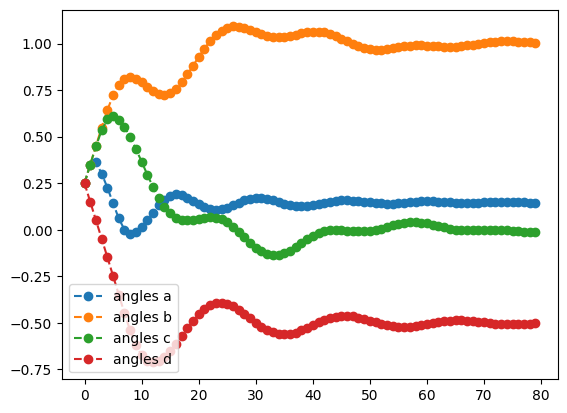
\includegraphics{index_files/figure-pdf/cell-8-output-2.pdf}

\includegraphics{index_files/figure-pdf/cell-8-output-3.pdf}

\includegraphics{index_files/figure-pdf/cell-8-output-4.pdf}

\includegraphics{index_files/figure-pdf/cell-8-output-5.pdf}

\includegraphics{index_files/figure-pdf/cell-8-output-6.pdf}

\includegraphics{index_files/figure-pdf/cell-8-output-7.pdf}

\includegraphics{index_files/figure-pdf/cell-8-output-8.pdf}

\includegraphics{index_files/figure-pdf/cell-8-output-9.pdf}

Building on this, we have gained some direct optimization protocols by
testing different concatenations of our excided state methods, including
the optimization after each of them. Of course, there are also other
possibilities of concatenations, since we have a lot of freedom in
choosing the suitable parameters and order of our excided state methods.


\printbibliography


\end{document}
